\chapter{Introduction}

La robotique est un domaine en plein essor. Depuis que le
superordinateur Deep Blue a battu Kasparov aux échecs en 1997, le
monde s'est rendu compte du potentiel de l'intelligence
artificielle.
\bigskip

Au-delà de la seule intelligence, le sport nécessite des capacités
physiques. Aussi, lors d'un match de football, l'environnement est
dynamique, il évolue sans cesse. Un robot qui joue au football se
voit donc davantage confronté à la complexité du monde réel.
\bigskip

La Robocup est une compétition où des robots autonomes
s'affrontent sur plusieurs disciplines. Depuis 1997, le tournoi de
football robotique est une discipline majeure du tournoi. 
Comme l'intelligence artificielle a surpassé l'homme aux échecs et
au jeu de Go, le but dans cette compétition est de créer une
équipe robotique capable de surpasser une équipe humaine.
\bigskip

Il existe d'autres matchs et tournois en dehors de cette
compétition, mais une victoire à la Robocup reste un enjeu majeur
pour les équipes.
\bigskip

Notre client est l'équipe \textbf{Rhoban}, évoluant dans la
compétition avec des robots humanoïdes kid-size, c'est à dire des
robots d'apparence humaine mesurant entre 40 et 90cm.
\bigskip

Notre but ici est de créer un outil d'annotation deafin de mieux
comprendre le match et les comportements des robots. À partir des
messages envoyés par les robots et d'un flux vidéo, nous allons
donc annoter les images en fonction de ce que le robot perçoit et
souhaite  faire.
\bigskip

Nous sommes capables d'annoter la position et la direction du
robot. On peut également incruster, pour un seul robot à la fois,
sa perception de la balle et l'historique de ses positions. Enfin,
nous sommes capables d'afficher la position que souhaite atteindre
un robot.
\bigskip

Nous proposons deux manières d'afficher la vidéo. Premièrement, un
outil simple permettant de visualiser une vidéo annotée selon des
paramètres prédéfinis par l'utilisateur.
\bigskip

Nous pouvons également afficher la vidéo dans une interface
graphique. Dans celle-ci, on peut gérer l'avancement de la lecture
grâce à un slider et changer les annotations en cours de
visionnage. 

On peut voir dans la Figure~\ref{fig:nonannote} une image de la
vidéo non annotée telle que fournie par le client :

\begin{figure}[H] 
\centering 
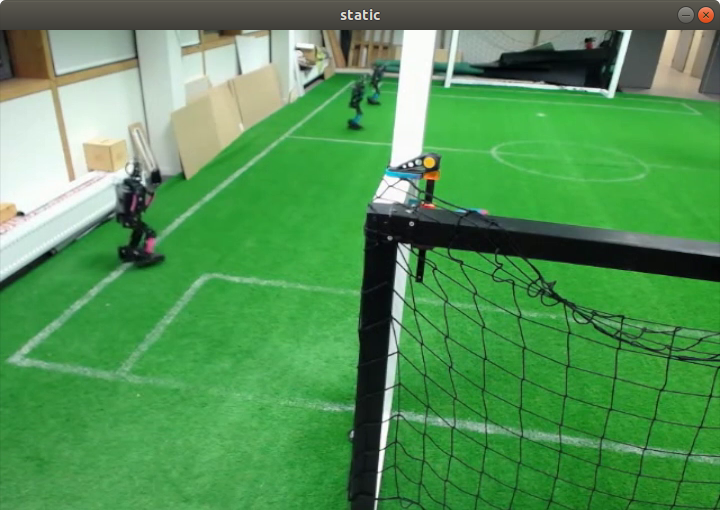
\includegraphics[scale = 0.25]{images/imagenonannote.png}
\caption{Image de la vidéo avant traitement}
\label{fig:nonannote}
\end{figure} 
\bigskip

Maintenant, on peut voir  dans la Figure~\ref{fig:annoted} une
image de la vidéo avec toutes les annotations proposées (sauf les
lignes du terrain, pour une meilleure visibilité). La balle (en
gris à gauche), la position souhaitée du robot (la croix et les
pointillés) ainsi que la trace (anciennes positions) sont celles
du robot 4 de l'équipe bleue.

\begin{figure}[H] 
\centering 
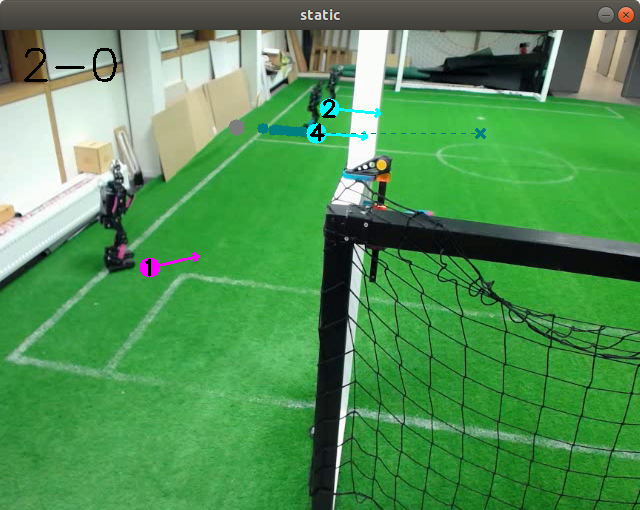
\includegraphics[scale = 0.25]{images/imageannote.png}
\caption{Image de la vidéo après traitement}
\label{fig:annoted}
\end{figure} 
\bigskip